\documentclass[a4paper,11pt]{exam}
%\printanswers % pour imprimer les réponses (corrigé)
\noprintanswers % Pour ne pas imprimer les réponses (énoncé)
\addpoints % Pour compter les points
% \noaddpoints % pour ne pas compter les points
\pointsinmargin
%\qformat{\textbf{\thequestion ) } }
%\qformat{\textbf{\thequestion )} \textit{\thepoints} \\  }  % Pour définir le style des questions (facultatif)
\usepackage{color} % définit une nouvelle couleur
\shadedsolutions % définit le style des réponses
% \framedsolutions % définit le style des réponses
\definecolor{SolutionColor}{rgb}{0.8,0.9,1} % bleu ciel
\renewcommand{\solutiontitle}{\noindent\textbf{Solution:}\par\noindent} % Définit le titre des solutions




\makeatletter

\def\maketitle{{\centering%
	\par{\huge\textbf{\@title}}%
	\par{\@date}%
	\par}}

\makeatother

\lhead{NOM Pr\'enom :}
\rhead{\textbf{Les r\'eponses doivent \^etre justifi\'ees}}
\cfoot{\thepage / \pageref{LastPage}}


%\usepackage{../../pas-math}
%\usepackage{../../moncours}


%\usepackage{pas-cours}
%-------------------------------------------------------------------------------
%          -Packages nécessaires pour écrire en Français et en UTF8-
%-------------------------------------------------------------------------------
\usepackage[utf8]{inputenc}
\usepackage[frenchb]{babel}
\usepackage[T1]{fontenc}
\usepackage{lmodern}
\usepackage{textcomp}



%-------------------------------------------------------------------------------

%-------------------------------------------------------------------------------
%                          -Outils de mise en forme-
%-------------------------------------------------------------------------------
\usepackage{hyperref}
\hypersetup{pdfstartview=XYZ}
%\usepackage{enumerate}
\usepackage{graphicx}
\usepackage{multicol}
\usepackage{tabularx}
\usepackage{multirow}


\usepackage{anysize} %%pour pouvoir mettre les marges qu'on veut
%\marginsize{2.5cm}{2.5cm}{2.5cm}{2.5cm}

\usepackage{indentfirst} %%pour que les premier paragraphes soient aussi indentés
\usepackage{verbatim}
\usepackage{enumitem}
\usepackage[usenames,dvipsnames,svgnames,table]{xcolor}

\usepackage{variations}

%-------------------------------------------------------------------------------


%-------------------------------------------------------------------------------
%                  -Nécessaires pour écrire des mathématiques-
%-------------------------------------------------------------------------------
\usepackage{amsfonts}
\usepackage{amssymb}
\usepackage{amsmath}
\usepackage{amsthm}
\usepackage{tikz}
\usepackage{xlop}
%-------------------------------------------------------------------------------



%-------------------------------------------------------------------------------


%-------------------------------------------------------------------------------
%                    - Mise en forme avancée
%-------------------------------------------------------------------------------

\usepackage{ifthen}
\usepackage{ifmtarg}


\newcommand{\ifTrue}[2]{\ifthenelse{\equal{#1}{true}}{#2}{$\qquad \qquad$}}

%-------------------------------------------------------------------------------

%-------------------------------------------------------------------------------
%                     -Mise en forme d'exercices-
%-------------------------------------------------------------------------------
%\newtheoremstyle{exostyle}
%{\topsep}% espace avant
%{\topsep}% espace apres
%{}% Police utilisee par le style de thm
%{}% Indentation (vide = aucune, \parindent = indentation paragraphe)
%{\bfseries}% Police du titre de thm
%{.}% Signe de ponctuation apres le titre du thm
%{ }% Espace apres le titre du thm (\newline = linebreak)
%{\thmname{#1}\thmnumber{ #2}\thmnote{. \normalfont{\textit{#3}}}}% composants du titre du thm : \thmname = nom du thm, \thmnumber = numéro du thm, \thmnote = sous-titre du thm

%\theoremstyle{exostyle}
%\newtheorem{exercice}{Exercice}
%
%\newenvironment{questions}{
%\begin{enumerate}[\hspace{12pt}\bfseries\itshape a.]}{\end{enumerate}
%} %mettre un 1 à la place du a si on veut des numéros au lieu de lettres pour les questions 
%-------------------------------------------------------------------------------

%-------------------------------------------------------------------------------
%                    - Mise en forme de tableaux -
%-------------------------------------------------------------------------------

\renewcommand{\arraystretch}{1.7}

\setlength{\tabcolsep}{1.2cm}

%-------------------------------------------------------------------------------



%-------------------------------------------------------------------------------
%                    - Racourcis d'écriture -
%-------------------------------------------------------------------------------

% Angles orientés (couples de vecteurs)
\newcommand{\aopp}[2]{(\vec{#1}, \vec{#2})} %Les deuc vecteurs sont positifs
\newcommand{\aopn}[2]{(\vec{#1}, -\vec{#2})} %Le second vecteur est négatif
\newcommand{\aonp}[2]{(-\vec{#1}, \vec{#2})} %Le premier vecteur est négatif
\newcommand{\aonn}[2]{(-\vec{#1}, -\vec{#2})} %Les deux vecteurs sont négatifs

%Ensembles mathématiques
\newcommand{\naturels}{\mathbb{N}} %Nombres naturels
\newcommand{\relatifs}{\mathbb{Z}} %Nombres relatifs
\newcommand{\rationnels}{\mathbb{Q}} %Nombres rationnels
\newcommand{\reels}{\mathbb{R}} %Nombres réels
\newcommand{\complexes}{\mathbb{C}} %Nombres complexes


%Intégration des parenthèses aux cosinus
\newcommand{\cosP}[1]{\cos\left(#1\right)}
\newcommand{\sinP}[1]{\sin\left(#1\right)}


%Probas stats
\newcommand{\stat}{statistique}
\newcommand{\stats}{statistiques}
%-------------------------------------------------------------------------------

%-------------------------------------------------------------------------------
%                    - Mise en page -
%-------------------------------------------------------------------------------

\newcommand{\twoCol}[1]{\begin{multicols}{2}#1\end{multicols}}


\setenumerate[1]{font=\bfseries,label=\textit{\alph*})}
\setenumerate[2]{font=\bfseries,label=\arabic*)}


%-------------------------------------------------------------------------------
%                    - Elements cours -
%-------------------------------------------------------------------------------





%\usepackage{fullpage}
\author{\ }
\date{24 Décembre 2017}
\title{Terminale ST$_2$S : DS num\'ero 2}


\begin{document}
%	\usepackage{fancyhdr}
%	
%	\pagestyle{fancy}
%	\fancyhf{}
	%\rhead{Share\LaTeX}

	\maketitle

\section{Un QCM (6 points)}

\textit{Cet exercice se présente sous la forme d'un questionnaire à choix multiple (QCM). Pour chaque question, trois réponses sont proposées. Une seule réponses est correcte. On demande de choisir celle que vous pensez être correcte.
}


On donne le tableau de variation d'une fonction $f$ définie et dérivable sur l'intervalle $[-12, 20]$ :

\begin{center}

	\begin{tikzpicture}[scale=0.8]
		\tkzTabInit{$x$/1.5,$f'(x)$/1.5,$f(x)$/4}{$-12$, $-5$, $7$, $20$}
		\tkzTabLine { ,- ,z , +, z, -}
		\tkzTabVar{+/$7$,-/$-4$,+/$-1$,-/$-6$}
	\end{tikzpicture}

\end{center}

\begin{questions}
	\question[1] On peut dire que :
	
		\begin{checkboxes}
			\choice $f$ est positive sur l'intervalle $[-12; -5]$.
			\choice $f$ est positive sur l'intervalle $[7; 20]$.
			\correctchoice $f$ est négative sur l'intervalle $[-5; 20]$.
		\end{checkboxes}
	
		
	\question[1] L'équation $f(x)=2$ possède 
	
	\begin{oneparcheckboxes}
		
		\correctchoice une seule solution ;
		\choice aucune solution ; 
		\choice on ne peut pas répondre.
	\end{oneparcheckboxes}	

	\question[1] On cherche à comparer $f'(0)$ et $f'(8)$ :

\begin{oneparcheckboxes}
	
	
	\choice $f'(0) < f'(8)$
	\correctchoice $f'(0) > f'(8)$
	\choice on ne peut pas répondre.
\end{oneparcheckboxes}

	\question[1] On cherche à comparer $f(0)$ et $f(8)$ :
	
	\begin{oneparcheckboxes}
		
		
		\choice $f(0) < f(8)$
		\choice $f(0) > f(8)$
		\correctchoice on ne peut pas répondre.
	\end{oneparcheckboxes}



	\question[1] Une équation de la tangente à la courbe représentative de la fonction $f$ au point d'abscisse 20 est :
	
	\begin{oneparcheckboxes}
		
		
		\choice $y = 20x - 6$
		\choice $y = -x - 6$
		\correctchoice $y = -x + 14$
	\end{oneparcheckboxes}

	\question[1] On désigne par $\mathcal{C}$ la courbe représentative de $f$ dans un repère orthogonal.
	
	\begin{oneparcheckboxes}
		
		\choice Il n'existe aucun point où la tangente à la courbe $\mathcal{C}$ est parallèle à l'axe des abscisses.
		\choice Il existe un seul point où la tangente à la courbe $\mathcal{C}$ est parallèle à l'axe des abscisses.
		\correctchoice Il existe deux points où la tangente à la courbe $\mathcal{C}$ est parallèle à l'axe des abscisses.
	\end{oneparcheckboxes}	
\end{questions}


\newpage

% Ajustement, taux d'évolution et tableur, suite géométrique

\section{Dépenses de santé (7 points)}

Le tableau suivant, extrait d'une feuille d'un tableur, donne la consommation de soins et de biens médicaux en milliards d'euros depuis l'année 2000.

\begin{center}
	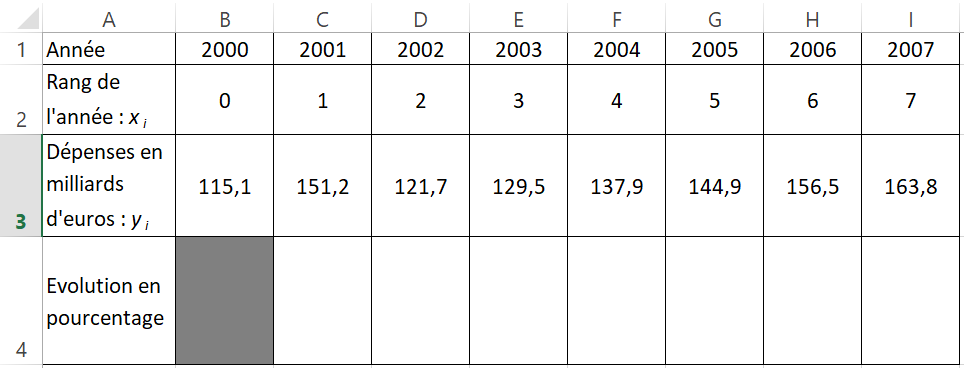
\includegraphics[scale=0.65]{img/biens_medicaux2}
\end{center}

\emph{Il n'est pas demandé de compléter le tableau.}

\subsection{Droite d'ajustement}

\begin{questions}
	\question[1] On suppose que la droite d'ajustement entre le rang de l'année $x$ et les dépenses en milliards d'euros $y$ a pour équation : $y = 7x + 115$. En utilisant cette équation, déterminer le montant des dépenses en 2010. 
	\begin{solution}
		L'année 2000 correspond au rang 0, donc le rang de l'année 2010 est 10. Calcul du montant des dépenses en 2010 :
		\begin{eqnarray*}
			y &=& 7x + 115 \\
			y &=& 7 \times 10 + 118 \\
			y &=& 188
		\end{eqnarray*}
	
	D'après l'équation de la droite d'ajustement, en 2010 les dépenses s'élèveront à 188 milliards d'euros.
	\end{solution}

\end{questions}

\subsection{Pourcentage d'évolution}

\begin{questions}
	\question[1] Quel est le pourcentage d'évolution global entre 2000 et 2007, à \num{0.1} \% prês ? 
	\begin{solution}
		\begin{eqnarray*}
			t &=& \dfrac{valeur d'arrivée - valeur de départ}{valeur de départ} \\
			t &=& \dfrac{\num{163.8} - \num{115.1}}{\num{115.1}} \\
			t &=& \dfrac{\num{48.7}}{\num{115.1}} \\
			t &=& \num{0.423}
		\end{eqnarray*}
	
		Soit une augmentation de \num{42.3} \% du montant des dépenses entre 2000 et 2007.
	\end{solution}

	\question[1] Quelle formule doit-on entrer en $C4$ pour déterminer le taux d'évolution des dépenses entre 2000 et 2001 et pouvoir la recopier vers la droite jusqu'en $I4$ ?
	\begin{solution}
		Pour déterminer le taux d'évolution des dépenses entre 2000 et 2001 il faut saisir la formule suivante en $C4$  :
		\begin{equation*}
			= (C3 - C2) / C3
		\end{equation*}
	\end{solution}
\end{questions}

\subsection{Limitation des dépenses}

Afin de mieux maîtriser les dépenses de santé, le gouvernement souhaitait, à partir de 2008, que les dépenses liées à la consommation de soins et de biens médicaux n'augmentent que de 2 \% par année. On modélise cette évolution par une suite. On désigne par $u_n$ le montant maîtrisé des dépenses pour l'année (2007 + $n$) en milliards d'euros. On a donc $u_0 = \num{163.8}$.

\begin{questions}
	\question[1] Calculer la valeur de $u_1$ (donner la valeur exacte).
	\begin{solution}
		Calcul de la valeur $u_1$ :
		\begin{eqnarray*}
			u_1 &=& u_O + \dfrac{u_0 \times 2}{100} \\
			u_1 &=& \num{163.8} + \dfrac{\num{163.8} \times 2}{100} \\
			u_1 &=& \num{163.8} + \num{3.276} \\
			u_1 &=& \num{167.076}
		\end{eqnarray*}
	\end{solution} 
	
	\question[1] Quelle est la nature de la suite $(u_n)$ ? On précisera les éléments caractéristiques de la suite.
	\begin{solution}
		Les dépenses liées à la consommation de soins et biens médicaux augmente de 2\% par an, donc chaque terme de la suite est obtenu est obtenu en multipliant le précédent par \num{1.02}.
		J'en déduis que $(u_n)$ est une suite géométrique de premier terme $u_0=\num{163.8}$ et de raison $q=\num{1.02}$.
	\end{solution}
	
	\question[1] Exprimer $u_n$ en fonction de $n$.
	\begin{solution}
		Expression de $u_n$ en fonction de $n$ :
		\begin{eqnarray*}
			u_n &=& u_0 \times q^n \\
			u_n &=& \num{163.8} \times \num{1.02}^n 
		\end{eqnarray*}
	\end{solution}
	
	\question[1] En supposant que cette modélisation reste valable jusqu'en 2015, à combien peut-on estimer le montant des dépenses en 2015 ? (Le résultat est à arrondir à $10^{-3}$).
	
	\begin{solution}
				
		$2015 = 2007 + 8$, donc pour estimer le montant des dépenses en 2015 il faut calculer la valeur du huitième terme de la suite, $u_8$ :
		
		\begin{eqnarray*}
			u_8 &=& \num{163.8} \times \num{1.02}^8 \\
			u_8 &\approx&  \num{191.918}\\
		\end{eqnarray*}
		
		On peut donc estimer le montant des dépenses en 2015 à  \num{191.918} milliards d'euros.
	\end{solution}
\end{questions}

  

%\newpage
	
%\section{Offres de prêt \textit{(8 points)}}

Une infirmière souhaitant créer un cabinet a besoin de d'un prêt de \num{100000} €. Elle contacte deux banques, A et B.\\


\begin{questions}
	\question La banque A lui propose un prêt remboursable en 7 annuités. Les annuités sont les termes consécutifs d'une suite arithmétique de premier terme $u_0 = \num{15000}$ (le premier remboursement est de \num{15000} €), et de raison \num{1800}.
	
	\begin{parts}
		\part[1] Calculer le montant des versements $u_1$, $u_2$, $u_3$, $u_4$, $u_5$ et $u_6$.
			\begin{solution}
				\begin{itemize}
					\item $u_1 = u_0 + \num{1800} = \num{15000} + \num{1800} = \num{16800}$;
					\item $u_2 = u_1 + \num{1800} = \num{16800} + \num{1800} = \num{18600}$;
					\item $u_3 = u_2 + \num{1800} = \num{18600} + \num{1800} = \num{20400}$;
					\item $u_4 = u_3 + \num{1800} = \num{20400} + \num{1800} = \num{22200}$;
					\item $u_5 = u_4 + \num{1800} = \num{22200} + \num{1800} = \num{24000}$;
					\item $u_6 = u_5 + \num{1800} = \num{24000} + \num{1800} = \num{25800}$.
				\end{itemize}
			\end{solution}
		\part[1\half] Quelle serait la somme totale remboursée si l'infirmière souscrivait le prêt auprès de la banque A ?\\
		
			\begin{solution}
				\begin{eqnarray*}
					S_n &=& \frac{(u_0 + u_n) \times (n +1)}{2} \\
					S_6 &=& \frac{(u_0 + u_6) \times 7}{2} \\
					S_6 &=& \frac{(\num{15000} + \num{25800}) \times 7}{2} \\
					S_6 &=& \frac{\num{39000} \times 7}{2} \\
					S_6 &=& \frac{\num{273000}}{2} \\
					S_6 &=& \num{136500} \\
				\end{eqnarray*}
				
				Si elle souscrivait le prêt auprès de la banque A, elle devrait rembourser \num{136500} €.
			\end{solution}
	\end{parts}

	\question La banque B propose également de rembourser le prêt sur 7 ans, en 7 versements. Le premier remboursement noté $v_0$ serait de \num{20000} €. Les remboursements suivants, notés $v_1$, $v_2$, $v_3$, $v_4$, $v_5$ et $v_6$ seraient chacun en augmentation de 2 \% par rapport au remboursement précédent.
	
	\begin{parts}
		\part[1] Calculer $v_1$ en précisant par quel calcul on passe de $v_0$ à $v_1$. Calculer $v_2$.
			\begin{solution}
				\begin{itemize}
					\item $ v_1 = v_0 \times \num{1.02} = \num{2000} \times \num{1.02} = \num{2040} $;
					\item $ v_2 = v_1 \times \num{1.02} = \num{2040} \times \num{1.02} = \num{2080.8} $.
				\end{itemize}
			\end{solution}
		
		\part[1] Donner pour tout entier $n$, $0 \leq n \leq 5$, l'expression de $v_{n+1}$ en fonction de $v_n$.
			\begin{solution}
				$v_{n+1} = v_n \times \num{1.02}$.
			\end{solution}
		
		\part[1] En déduire que les nombres $v_0$, ..., $v_6$ sont des termes consécutifs d'une suite géométrique de premier terme $v_0$ dont on précisera la raison $q$.
			\begin{solution}
				Pour passer d'un terme à l'autre, on multiplie toujours par \num{1.02}, donc $ (v_n)$ est une suite géométrique de raison $q = \num{1.02}$.
			\end{solution}
		
		\part[1\half] Quelle serait la somme totale remboursée si l'infirmière souscrivait le prêt auprès de la banque B ? Arrondir à l'euro.\\
			\begin{solution}
				\begin{eqnarray*}
					S_n &=& v_0  \times \frac{1 - q^{n+1}}{1 - q} \\
					S_6 &=& \num{20000}  \times \frac{1 - \num{1.02}^{7}}{1 - \num{1.02}} \\
					S_6 &=& \num{148686} 
				\end{eqnarray*}
				
				Si elle souscrivait le prêt auprès de la banque A, elle devrait rembourser \num{148686} €.
			\end{solution}
	\end{parts}

	\question[1] Quelle banque offre la solution la plus avantageuse ?
	
		\begin{solution}
			\num{136500} < \num{148686}, donc la banque A est plus avantageuse que la banque B.
		\end{solution}
\end{questions}

	\label{LastPage}
	

\end{document}